\section{Zielsetzung}
Ziel des Versuches ist es, den Wirkungsgrad bzw. die Kenngrößen 
einer Wärmepumpe zu bestimmen.
\section{Theorie}
\label{sec:Theorie}

Das System einer Wärmepumpe besteht aus zwei Reservoiren, die 
während des Betriebs der Pumpe verschiedene Temeperaturen aufweisen.
Thermodynamische Beobachtungen zeigen, dass sich, in einem abgeschlossenen
System, die Wärmeenergie immer von warm zu kalt begibt. Diesen
Prozess umzukehren bewirkt die Wärmepumpe. Dies kann jedoch nur mit 
verrichteter Arbeit geschehen. Um den Wirkungsgrad einer Wärmepumpe 
zu quantifizieren, wird die Güteziffer $\nu$ eingeführt. Sie wird 
über den ersten Hauptsatz der Thermodynamik hergeleitet und berechnet 
sich über 
\begin{equation}
    \nu=Q_1/A\,.
\end{equation}
Dabei ist $Q_1$ die vom Transportmedium an das wärmere Reservoir abegebene
Wärme und $A$ die dafür verwendete Arbeit. $\nu$ stellt also das Verhältnis 
zwischen übergebener Wärme und dafür benötigter Arbeit dar. Nach dem zweiten
Hauptsatz der Thermodynamik lässt sich folgender idealisierter Ausdruck für 
das Verhältnis der übertragenen Wärme und deren Temperaturen herleiten 
\begin{equation}
    \frac{Q_1}{T_1}-\frac{Q_2}{T_2}=0\,.
\end{equation}
Da hierfür gefordert ist, dass die Wärmeübertagung sowie die dafür aufgewandte
Arbeit komplett reversibel sei, gilt für reale Systeme 
\begin{equation}
    \frac{Q_1}{T_1}-\frac{Q_2}{T_2}>0\,.
\end{equation}
Aus diesen Feststellungen lässt sich für die ideale und reale Güteziffer der 
Ausdruck 
\begin{align}
    \nu_\text{ideal}&=\frac{Q_1}{A}=\frac{T_1}{T_1-T_2} \label{eq:Gueteideal}\\
    \nu_\text{real}&<\frac{T_1}{T_1-T_2}
\end{align}
finden. Aus diesen Ausdrücken ist zu erkennen, dass eine Wärmepumpe bei kleinen 
Temperaturdifferenzen einen höheren Wirkunsgrad hat als bei großen.
Die von der Wärmepumpe transportierte Energie ist eine Phasenumwandlungsenergie. 
Das bedeutet, dass das als Transportmedium verwendete Gas beim Verdampfen Wärme 
aufnimmt und diese beim Kondensieren wieder abgibt, worin schließlich die
Energieübertragung liegt. In \autoref{fig:Messapparatur} ist der Aufbau einer
\begin{figure}
    \centering
    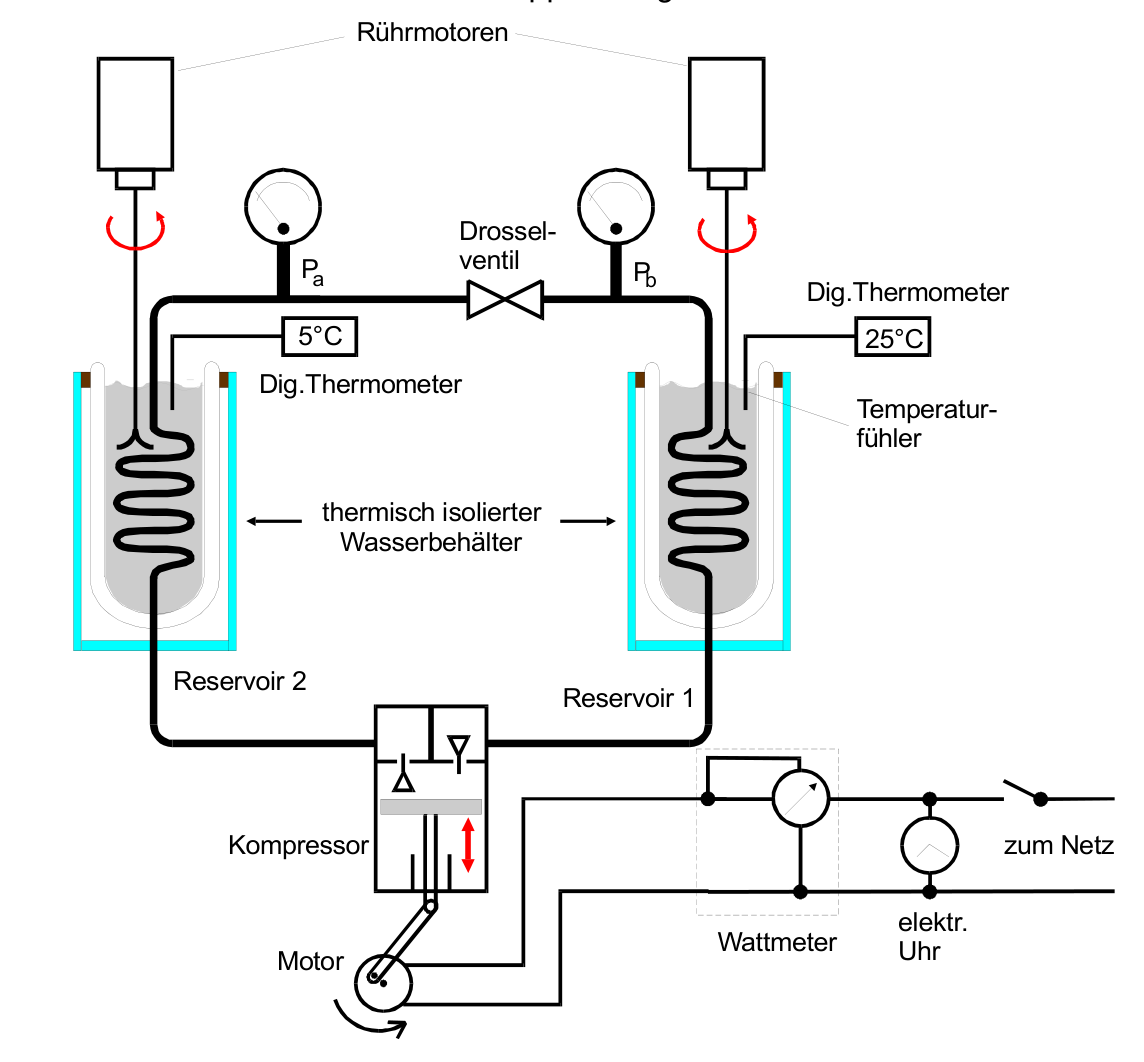
\includegraphics[height=8cm]{messdaten/Messapparatur.png}
    \caption{Die im Versuch verwendete Messapparatur der Wärmepumpe. \cite{V206_Anleitung}}
    \label{fig:Messapparatur}
\end{figure}
Wärmepumpe, sowie die zum Durchführen des Versuchs nötigen Anbauten skizziert.
Zunächst wird am flüssigen Teil des Mediums die Temeperatur $T_1$ sowie der Druck
$p_\text{b}$ gemessen. Nach Durchfließens des Dorsselventils $D$ verdampft die 
Flüssigkeit und es werden die Temeperatur $T_2$ sowie der Druck $p_\text{a}$ 
gemessen. Dabei werden die Temeperaturen jeweils in einem Reservoir gefüllt mit 
Wasser gemessen, durch das sich spiralenförmig Leitungen, gefüllt mit dem Transportmedium,
befinden. Um die Temeperatur im jeweils ganzen Reservoir konstant zu halten, sind in beiden 
Rührmotoren eingebaut, um das Wasser ständig zu mischen. Die jeweils übertragene Energie
wird in Kondensations- bzw. Verdampfungswärme $L$ pro Gramm Stoff angegeben.
Wichtig für den realen Betrieb ist außerdem der Reiniger $R$, der dafür sorgt dass die
Flüssigkeit frei von Gasbläschen ist. Anderesherum sorgt die Steuereinheit $S$ dafür,
dass nur reines Gas ohne Flüssigkeit in den Kompressor gelangt.
Um die schon definierte reale Güteziffer aus einer Messreihe der Temeperatur in 
Abhängigkeit der Zeit zu bestimmen, wird erst die pro Zeit gewonnen Wärmemenge definiert mit
\begin{equation}
    \frac{\increment Q_1}{\increment t}=(m_1c_\text{w}+m_\text{k}c_\text{k})\frac{\increment T_1}{\increment t}\,.
\end{equation}
Die Wärmekapazität des Kupferrohrs sowie des Eimers werden durch $m_\text{k}c_\text{k}$ beschrieben,
die Wärmekapazität des Wassers im ersten Reservoir durch $m_1c_\text{w}$\,.
Mit der neuen Variable $N$, welche die über $\increment t$ zeitlich gemittelte Leistung des 
Wattmeters angibt, ergibt sich für die Güteziffer 
\begin{equation}
    \nu=\frac{\increment Q_1}{\increment t\,N}\,.
    \label{eq:Guetereal}
\end{equation}
Analog zur ersten Temperaturmessung ergibt sich für die zweite Temperaturmessung
\begin{equation}
    \frac{\increment Q_2}{\increment t}=(m_2c_\text{w}+m_\text{k}c_\text{k})\frac{\increment T_2}{\increment t}
\end{equation}
als Differenzenqueotient. Daraus ergibt sich bei bekannter Verdampfungswärme $L$ eine Formel,
aus der sich der Massendurchsatz bestimmen lässt
\begin{equation}
    \frac{\increment Q_2}{\increment t}=L\frac{\increment m}{\increment t}\,.
    \label{eq:massendurchsatz}
\end{equation}
Für die Arbeit $A_\text{m}$, welche der Kompressor leisten muss, um ein Gasvolumen von $V_\text{a}$
auf $V_\text{b}$ zu verringen, gilt 
\begin{equation}
    A_\text{m}=-\int_{V_\text{a}}^{V_\text{b}}p \,\text{d} V\,.
\end{equation}
Über die Annahme, die Kompression verlaufe adiabatisch und den damit geltenen Poissonsche Gleichung
ergibt sich für die mechanische Kompressorleistung
\begin{equation}
N_\text{mechanisch}=\frac{\increment A_\text{m}}{\increment t}=\frac{1}{\kappa-1}\left(p_\text{b}
\sqrt{\frac{p_\text{a}}{p_\text{b}}}-p_\text{a}\right)\frac{1}{\rho}\frac{\increment m}{\increment t}\,.
\label{eq:mechanisch}
\end{equation}
Bei Druck $p_\text{a}$ ist $\rho$ die Dichte des gasförmigen Tansportmediums.

